% Files using this must be two subfolders
% deep. Adjust the number of ../ for the
% depth of the file.
% Imports
\usepackage{fancyhdr}
\usepackage{geometry}
\usepackage{icomma}
\usepackage{amsmath}
\usepackage{multicol}
\usepackage{mathptmx}
\usepackage{anyfontsize}
\usepackage{t1enc}
\usepackage{tabto}
\usepackage{listings}
\usepackage{filecontents}
\usepackage{subcaption}
\usepackage{tikz}
\usepackage[parfill]{parskip}
\usepackage{graphicx}
\usepackage[]{mdframed}
\usepackage{amsmath}
\usepackage[makeroom]{cancel}
\usepackage{pgfplots}
\usepackage{pgfplotstable}
\usepackage{xfrac}
\usepackage{amssymb}
\usepackage{mathtools}
\pgfplotsset{compat=1.18}
\usetikzlibrary{patterns}
\usepgfplotslibrary{polar}
\usepgfplotslibrary{fillbetween}

\geometry{margin=2.5cm}

\newcommand{\name}{Kaleb Burris}
\newcommand{\classname}{MATH F253, Elizabeth S. Allman, University of Alaska Fairbanks}
\newcommand{\assignment}{FILL IN ASSIGNMENT NAME}

\pagestyle{fancy}

\fancyhead[L]{
    \name 
    \newline
    \classname
    \newline
    \assignment
}

\newcommand{\horizontal}{\noindent\rule{\hsize}{0.4pt}}

\setlength{\headheight}{42pt}
\setlength{\headsep}{0.25in}
\setlength{\columnsep}{0.35cm}
\setlength{\columnseprule}{1pt}

\usepackage[T1]{fontenc}
\usepackage{lmodern}

% Put class number, class name, and professor 
% name.
% Use only in case of emergency, this
% should be covered by the preamble.
% \renewcommand\classname{}

% Put the assignment name with \S if 
% necessary for the section and the question 
% numbers.
\renewcommand\assignment{Homework Set IV, Due February 2, 2023: \S 2.3 \# 122, 124, 130}

\begin{document}
    % Templates
    \iffalse
    % Use these for equations.
    \begin{equation*}
        \begin{gathered}
            Equations go here.
        \end{gathered}
    \end{equation*}

    % Use this if a line of math is too long.
    \resizebox{\hsize}{!}{$Long equation goes here$}

    % Use these for multiple columns.
    \begin{multicol*}{# of columns}
        % Remove the * if you want the columns to be balanced.
    \end{multicol*}

    % Use this to add a horizontal line.
    \horizontal

    \fi

    % Begin homework here.
    %%%%%%%%%%%%%%%%%%%%%%

    \subparagraph*{122.} $y = \frac{1}{x}, \quad x = 1, \quad \text{and} \quad x = 100$

    \begin{multicols}{2} 
        \centering\begin{tikzpicture}[scale=0.8]
            \begin{axis}[
                axis lines=middle,
                axis line style={->},
                xlabel={$x$},
                ylabel={$y$},
                no markers,
                ymin=0, ymax=1,
                xmin=-0,   xmax=100
            ]
                \fill [pattern=north east lines, pattern color=black, domain=1:100, variable=\x]
                (1, 0)
                -- plot ({\x}, {1/\x})
                -- (100, 0)
                -- cycle;
                \addplot[samples=100, domain=0:100]{1/x};
            \end{axis}
        \end{tikzpicture}

        \columnbreak

        \begin{align*}
            V & = 2\pi\int_{1}^{100}\left(\frac{1}{x}\right)\mathrm{d}x  \\
              & = 2\pi\ln(x)\Big|_{1}^{100}                              \\
              & = 2\pi(\ln(100) - \ln(1))                                \\
              & = \boxed{2\pi\ln(100)}
        \end{align*}
    \end{multicols}

    \horizontal

    \paragraph*{124.}
    $y=\frac{1}{1+x^2}, \quad x=0, \quad \text{and} \quad x=3$

    \begin{multicols}{2} 
        \centering\begin{tikzpicture}[scale=0.8]
            \begin{axis}[
                axis lines=middle,
                axis line style={->},
                xlabel={$x$},
                ylabel={$y$},
                no markers,
                ymin=0, ymax=1.5,
                xmin=0,   xmax=4
            ]
                \fill [pattern=north east lines, pattern color=black, domain=0:3, variable=\x]
                (0, 0)
                -- plot ({\x}, {1/(1+\x*\x)})
                -- (3, 0)
                -- cycle;
                \addplot[samples=100, domain=0:3]{1/(1+x^2)};
                \draw (3,0) -- (3,3);
            \end{axis}
        \end{tikzpicture}

        \columnbreak

        \begin{align*}
            V & = 2\pi\int_{0}^{3}\left(\frac{1}{1+x^2}\right)\mathrm{d}x   \\
              & = 2\pi\tan^{-1}(x)\Big|_{1}^{3}                             \\
              & = \boxed{2\pi[\tan^{-1}(3) - \tan^{-1}(1)]}
        \end{align*}
    \end{multicols}

    \horizontal

    \paragraph*{130.}
    $y=\sqrt{1-x^2}, \quad x=0, \quad \text{and} \quad x=1$

    \begin{multicols}{2} 
        \centering\begin{tikzpicture}[scale=0.8]
            \begin{axis}[
                axis lines=middle,
                axis line style={->},
                xlabel={$x$},
                ylabel={$y$},
                no markers,
                ymin=0, ymax=1.5,
                xmin=0,   xmax=1.5
            ]
                \fill [pattern=north east lines, pattern color=black, domain=0:1, variable=\x]
                (0, 0)
                -- plot ({\x}, {(1-\x^2)^0.5})
                -- (1, 0)
                -- cycle;
                \addplot[samples=100, domain=0:1]{(1-x^2)^(1/2)};
                \draw (3,0) -- (3,3);
            \end{axis}
        \end{tikzpicture}

        \columnbreak
        \begin{equation*}
            \resizebox*{0.5\textwidth}{!}{$
            \begin{gathered}
                V = 2\pi\int_{0}^{1}\left(\sqrt{1-x^2}\right)\mathrm{d}x   \\
                \text{Using} \quad a^2-u^2 \quad \rightarrow \quad u = a\sin \theta, \quad \mathrm{d}u = a\cos \theta \mathrm{d}\theta  \\
                x = \sin \theta, \quad \mathrm{d}x = \cos\theta \mathrm{d}\theta \quad \theta = \sin^{-1}x    \\
                \Rightarrow V = 2\pi\int\left(\sqrt{1-\sin^{2}\theta}\cos\theta\right)\mathrm{d}\theta   \\
                = 2\pi\int\left(\sqrt{\cos^{2}\theta}\cos\theta\right)\mathrm{d}\theta = 2\pi\int(\cos^{2}\theta)\mathrm{d}\theta  \\
                = 2\pi\int\left(\frac{1+\cos\theta}{2}\right)\mathrm{d}\theta \implies 2\pi\left(\frac{\theta+\sin\theta}{2}\right) \implies 2\pi\left.\left(\frac{\sin^{-1}x+\sin\sin^{-1}x}{2}\right)\right|_{0}^{1}  \\
                = 2\pi\left(\frac{\frac{\pi}{2}+1 - 0}{2}\right) = 2\pi\left(\frac{\frac{2\pi}{2}}{2}\right) = \boxed{\frac{\pi}{4}}
            \end{gathered}$}
        \end{equation*}
    \end{multicols}

\end{document}